\chapter{Kodierungen}

Wir haben in den vorausgegangenen Kapiteln gelernt, wie man Zahlen im Binärsystem sowie in anderen $b$-adischen Systemen darstellt. Wir möchten jedoch selbstverständlich nicht nur Zahlen, sondern auch andere digitale Informationen wie etwa Buchstaben oder Bilder darstellen können. Im folgenden Kapitel widmen wir uns daher der Darstellung von Buchstaben und Bildern, sowie weiteren Dateiformaten im Allgemeinen.

\section{Bits und Bytes}
In Computern treten Bits oft in 8er-Gruppen auf. Einen solchen Block von 8 Bits nennt man ein Byte. Der Ausdruck stammt aus dem Englischen und setzt sich aus einem Wortspiel von \textit{bit} ($=$ \textit{\underline{bi}nary digi\underline{t}}), \enquote{binäre Ziffer}, und \textit{bite} = \enquote{Bissen} zusammen (die Schreibweise \enquote{byte} wurde gewählt, um eine Verwechslung mit dem englischen Wort \textit{bite} zu vermeiden).

Folgende Zahl ist die binäre Repräsentation der Dezimalzahl 22:

\[00010110_2 = 22_{10}\]

Bei Dezimalzahlen sind wir daran gewohnt, führende Nullen einfach wegzulassen (man könnte schliesslich genauso gut 000022 schreiben) -- bei Binärzahlen werden üblicherweise alle Bits ausgeschrieben (also 00010110, nicht 10110).

\begin{myexercise}
	Wie wird die Zahl $42_{10}$ mit einem Byte dargestellt? Vergessen Sie die führenden Nullen nicht!
	\begin{myanswer}
		$00101010_2$
	\end{myanswer}
\end{myexercise}

\begin{myexercise}
	\label{ex:byte-max}
	Welches ist die grösste Dezimalzahl, die mit einem Byte ($=$ 8 Bits) ausgedrückt werden kann?
	\begin{myanswer}
		$255_{10} = 11111111_2$
	\end{myanswer}
\end{myexercise}

\section{Kodierung von Buchstaben: ASCII-Tabellen und UTF-8}
In den vorausgehenden Kapiteln haben wir gelernt, dass Zahlen in unterschiedlichen Zahlensystemen unterschiedlich repräsentiert werden können. Insbesondere haben wir uns das Binärsystem genauer angeschaut, da elektronische Rechner typischerweise Informationen in binärer Form verarbeiten.

Wenn Computer lediglich Nullen und Einsen abspeichern können, wie kann man damit Zahlen und Buchstaben repräsentieren? Genau dies wurde umgesetzt mit einer der ersten \tib{Text-Kodierungen}, dem \gls{ASCII}.

Die Grundidee der \gls{ASCII}-Kodierung war, ein Byte pro Zeichen zu verwenden. Ein Bit war allerdings reserviert für weitere Zwecke, wie beispielsweise die Fehlerkorrektur (Paritätsbit). Daher stehen in der originalen ASCII-Kodierung lediglich 7 Bits zur Kodierung von Buchstaben zur Verfügung.

\begin{myexercise}
	Wie viele unterschiedliche Zeichen kann man mit der ASCII-Kodierung abbilden, wenn man nur 7 von 8 Bits zur Kodierung nutzt?
	\begin{myanswer}
		128 Zeichen, da $2^7=128$.
	\end{myanswer}
\end{myexercise}
\begin{myexercise}
	Welches ist die grösste binäre Zahl, die man mit 8 Bits (einem Byte) darstellen kann? Wie lautet diese Zahl in hexadezimaler Darstellung?
	\begin{myanswer}
		Die grösste binäre Zahl mit 8 Bits ist $11111111_2 = 255_{10} = FF_{16}$. Wir sehen also, dass man mit lediglich zwei Ziffern alle binären Codes eines Bytes darstellen kann. Unter anderem wird auch aus diesem Grund häufig die hexadezimale Darstellung für Byte-Codes verwendet.
	\end{myanswer}
\end{myexercise}

Leider reichen die wenigen Zeichen, welche mit dem \gls{ASCII}-Standard kodiert werden können, bei weitem nicht aus, um die Vielfalt an heutigen Zeichen (in unterschiedlichen Sprachen), Spezialzeichen und Emojis darzustellen -- daher wurde \gls{ASCII} mittlerweile auf breiter Front von einem neuen Standard abgelöst -- \gls{UTF-8}. Bei diesem Standard stehen für jedes Zeichen bis zu 4 Bytes zur Verfügung.
\begin{myexercise}
	Wie viele unterschiedliche Zeichen kann man mit vier Bytes maximal abbilden?
	\begin{myanswer}
		$2^{32}=$4'294'967'296 mögliche Zeichen. Allerdings kann UTF-8 etwas weniger Zeichen abbilden, da im ersten Byte noch Speicherplatz eingerechnet werden muss zur Angabe, ob das Zeichen mit 1, 2, 3 oder 4 Bytes angegeben wird.
	\end{myanswer}
\end{myexercise}


\clearpage

\begin{table}[H]
	\centering
	\resizebox{!}{.35\paperheight}{
		\begin{tabular}{c||c}
			\rowcolors{2}{gray!25}{white}
			\begin{tabular}{cccc}
				\toprule
				Dezimal & Hexadezimal & Binär    & Zeichen \\
				\midrule
				0       & 00          & 00000000 & NUL     \\
				1       & 01          & 00000001 & SOH     \\
				2       & 02          & 00000010 & STX     \\
				3       & 03          & 00000011 & ETX     \\
				4       & 04          & 00000100 & EOT     \\
				5       & 05          & 00000101 & ENQ     \\
				6       & 06          & 00000110 & ACK     \\
				7       & 07          & 00000111 & BEL     \\
				8       & 08          & 00001000 & BS      \\
				9       & 09          & 00001001 & HT      \\
				10      & 0A          & 00001010 & LF      \\
				11      & 0B          & 00001011 & VT      \\
				12      & 0C          & 00001100 & FF      \\
				13      & 0D          & 00001101 & CR      \\
				14      & 0E          & 00001110 & SO      \\
				15      & 0F          & 00001111 & SI      \\
				16      & 10          & 00010000 & DLE     \\
				17      & 11          & 00010001 & DC1     \\
				18      & 12          & 00010010 & DC2     \\
				19      & 13          & 00010011 & DC3     \\
				20      & 14          & 00010100 & DC4     \\
				21      & 15          & 00010101 & NAK     \\
				22      & 16          & 00010110 & SYN     \\
				23      & 17          & 00010111 & ETB     \\
				24      & 18          & 00011000 & CAN     \\
				25      & 19          & 00011001 & EM      \\
				26      & 1A          & 00011010 & SUB     \\
				27      & 1B          & 00011011 & ESC     \\
				28      & 1C          & 00011100 & FS      \\
				29      & 1D          & 00011101 & GS      \\
				30      & 1E          & 00011110 & RS      \\
				31      & 1F          & 00011111 & US      \\
				32      & 20          & 00100000 & Space   \\
				33      & 21          & 00100001 & !       \\
				34      & 22          & 00100010 & "       \\
				35      & 23          & 00100011 & \#      \\
				36      & 24          & 00100100 & \$      \\
				37      & 25          & 00100101 & \%      \\
				38      & 26          & 00100110 & \&      \\
				39      & 27          & 00100111 & '       \\
				40      & 28          & 00101000 & (       \\
				41      & 29          & 00101001 & )       \\
				42      & 2A          & 00101010 & *       \\
				43      & 2B          & 00101011 & +       \\
				44      & 2C          & 00101100 & ,       \\
				45      & 2D          & 00101101 & -       \\
				46      & 2E          & 00101110 & .       \\
				47      & 2F          & 00101111 & /       \\
				48      & 30          & 00110000 & 0       \\
				49      & 31          & 00110001 & 1       \\
				50      & 32          & 00110010 & 2       \\
				51      & 33          & 00110011 & 3       \\
				52      & 34          & 00110100 & 4       \\
				53      & 35          & 00110101 & 5       \\
				54      & 36          & 00110110 & 6       \\
				55      & 37          & 00110111 & 7       \\
				56      & 38          & 00111000 & 8       \\
				57      & 39          & 00111001 & 9       \\
				58      & 3A          & 00111010 & :       \\
				59      & 3B          & 00111011 & ;       \\
				60      & 3C          & 00111100 & <       \\
				61      & 3D          & 00111101 & =       \\
				62      & 3E          & 00111110 & >       \\
				63      & 3F          & 00111111 & ?       \\\bottomrule
			\end{tabular} &
			\rowcolors{2}{gray!25}{white}
			\begin{tabular}{cccc}
				\toprule
				Dezimal & Hexadezimal & Binär    & Zeichen         \\
				\midrule

				64      & 40          & 01000000 & @               \\
				65      & 41          & 01000001 & A               \\
				66      & 42          & 01000010 & B               \\
				67      & 43          & 01000011 & C               \\
				68      & 44          & 01000100 & D               \\
				69      & 45          & 01000101 & E               \\
				70      & 46          & 01000110 & F               \\
				71      & 47          & 01000111 & G               \\
				72      & 48          & 01001000 & H               \\
				73      & 49          & 01001001 & I               \\
				74      & 4A          & 01001010 & J               \\
				75      & 4B          & 01001011 & K               \\
				76      & 4C          & 01001100 & L               \\
				77      & 4D          & 01001101 & M               \\
				78      & 4E          & 01001110 & N               \\
				79      & 4F          & 01001111 & O               \\
				80      & 50          & 01010000 & P               \\
				81      & 51          & 01010001 & Q               \\
				82      & 52          & 01010010 & R               \\
				83      & 53          & 01010011 & S               \\
				84      & 54          & 01010100 & T               \\
				85      & 55          & 01010101 & U               \\
				86      & 56          & 01010110 & V               \\
				87      & 57          & 01010111 & W               \\
				88      & 58          & 01011000 & X               \\
				89      & 59          & 01011001 & Y               \\
				90      & 5A          & 01011010 & Z               \\
				91      & 5B          & 01011011 & [               \\
				92      & 5C          & 01011100 & \textbackslash  \\
				93      & 5D          & 01011101 & ]               \\
				94      & 5E          & 01011110 & \^{}            \\
				95      & 5F          & 01011111 & \_              \\
				96      & 60          & 01100000 & `               \\
				97      & 61          & 01100001 & a               \\
				98      & 62          & 01100010 & b               \\
				99      & 63          & 01100011 & c               \\
				100     & 64          & 01100100 & d               \\
				101     & 65          & 01100101 & e               \\
				102     & 66          & 01100110 & f               \\
				103     & 67          & 01100111 & g               \\
				104     & 68          & 01101000 & h               \\
				105     & 69          & 01101001 & i               \\
				106     & 6A          & 01101010 & j               \\
				107     & 6B          & 01101011 & k               \\
				108     & 6C          & 01101100 & l               \\
				109     & 6D          & 01101101 & m               \\
				110     & 6E          & 01101110 & n               \\
				111     & 6F          & 01101111 & o               \\
				112     & 70          & 01110000 & p               \\
				113     & 71          & 01110001 & q               \\
				114     & 72          & 01110010 & r               \\
				115     & 73          & 01110011 & s               \\
				116     & 74          & 01110100 & t               \\
				117     & 75          & 01110101 & u               \\
				118     & 76          & 01110110 & v               \\
				119     & 77          & 01110111 & w               \\
				120     & 78          & 01111000 & x               \\
				121     & 79          & 01111001 & y               \\
				122     & 7A          & 01111010 & z               \\
				123     & 7B          & 01111011 & \{              \\
				124     & 7C          & 01111100 & |               \\
				125     & 7D          & 01111101 & \}              \\
				126     & 7E          & 01111110 & \textasciitilde \\
				127     & 7F          & 01111111 & DEL             \\
				\bottomrule
			\end{tabular}
		\end{tabular}}
	\caption{Darstellbare Zeichen der originalen \gls{ASCII}-Kodierung}
	\label{table:ascii}
\end{table}
\clearpage

\begin{myexercise}
	Im Computer ist die folgende Bit-Folge gespeichert:

	\texttt{01101000 01100101 01101100 01101100 01101111}

	Nutzen Sie \cref{table:ascii}, um die Bit-Folge in Zeichen zu übersetzen. Welches Wort wird damit codiert?

	\textbf{Tipp}: Nutzen Sie die Suchfunktion (\keys{\ctrl + F}, oder \keys{\cmd + F}) um in der ASCII-Tabelle nach den Bitfolgen zu suchen.
	\begin{myanswer}
		hello
	\end{myanswer}
\end{myexercise}

\begin{myexercise}
	Schreiben Sie Ihren Namen in der \gls{ASCII}-Kodierung.
\end{myexercise}

\section{Kodierung von Bildern}

Auch Bilder werden im Computer durch Nullen und Einsen repräsentiert, üblicherweise indem die einzelnen Bildpunkte ($=$ Pixel) in eine bestimmte Ordnung gebracht werden (meist Durchzählen von links nach rechts, dann von oben nach unten), und für jedes Pixel wird dann einfach ein Farbwert gespeichert -- also eine (Binär-)Zahl die angibt, welche Farbe dieses Pixel hat.

Wenn es sich um ein Schwarz-Weiss-Bild handelt ist dies relativ einfach, wie \cref{table:bw-img} zeigt.

\begin{table}[H]
	\centering
	\begin{tabular}{lllll}
		1 & 0 & 0 & 0 & 1 \\
		0 & 1 & 0 & 1 & 0 \\
		0 & 0 & 1 & 0 & 0 \\
		0 & 1 & 0 & 1 & 0 \\
		1 & 0 & 0 & 0 & 1
	\end{tabular}
	\caption{Beispiel eines Schwarz-Weiss-Bilds}
	\label{table:bw-img}
\end{table}

\begin{myexercise}
	Um was für ein Bild handelt es sich bei \cref{table:bw-img}?
	\begin{myanswer}
		Um ein Kreuz.
	\end{myanswer}
\end{myexercise}

\begin{myexercise}
	Wie viele Bit Speicherplatz benötigt das Bild?
	\begin{myanswer}
		25 ($= 5\cdot 5$).
	\end{myanswer}
\end{myexercise}

\begin{myexercise}
	Angenommen, für jeden Pixel stünden nicht nur Schwarz und Weiss, sondern insgesamt 8 Graustufen zur Verfügung. Wie viel Speicherplatz (in Bits) wäre dann nötig, um das Bild zu speichern?
	\begin{myanswer}
		75, da 3 Bits ausreichen, um 8 verschiedene Stufen abzubilden (von 0 bis 7, $7_{10}=111_2$). Daher haben wir 3 Bits * 25 Pixel = 75 Bits.
	\end{myanswer}
\end{myexercise}

\begin{myexercise}
	\gls{GIF}-Bilder im Internet können in der Regel 256 Farben unterscheiden. Wie viele Bits pro Pixel sind dafür nötig?
	\begin{myanswer}
		8 (siehe Lösung auf \cref{ex:byte-max}). Hierbei werden nicht wie üblich dieselbe Anzahl Bits pro Farbe verwendet, sondern es wird ein sogenannter \tib{Index} verwendet, der auf eine Farbpalette verweist. In der Farbpalette werden die 256 Farben definiert, und jedes Pixel speichert lediglich den Index (also die Position) der Farbe in der Palette. Daher reicht es, 8 Bits pro Pixel zu verwenden, um die 256 möglichen Farben zu kodieren.
	\end{myanswer}
\end{myexercise}

\section{Kodierung von Farben}
Computerbildschirme bestehen aus sogenannten Pixeln, welche aus winzigen Lampen bestehen (typischerweise in \gls{LED}-Technologie), die entweder rot, grün oder blau leuchten können. Das Wort Pixel setzt sich aus den englischen Begriffen \enquote{picture} (Bild) und \enquote{element} (Element) zusammen. Es bezeichnet also das kleinste Bildelement eines digitalen Bildes oder Bildschirms. Jeder Pixel stellt einen einzelnen Punkt dar, dessen Farbe und Helligkeit individuell gesteuert werden kann. Falls Sie zu Hause einen alten Bildschirm haben, können Sie den gerne von nahe betrachten und sollten die einzelnen \glspl{LED} erkennen können (siehe \cref{fig:pixels}).

\begin{figure}[H]
	\centering
	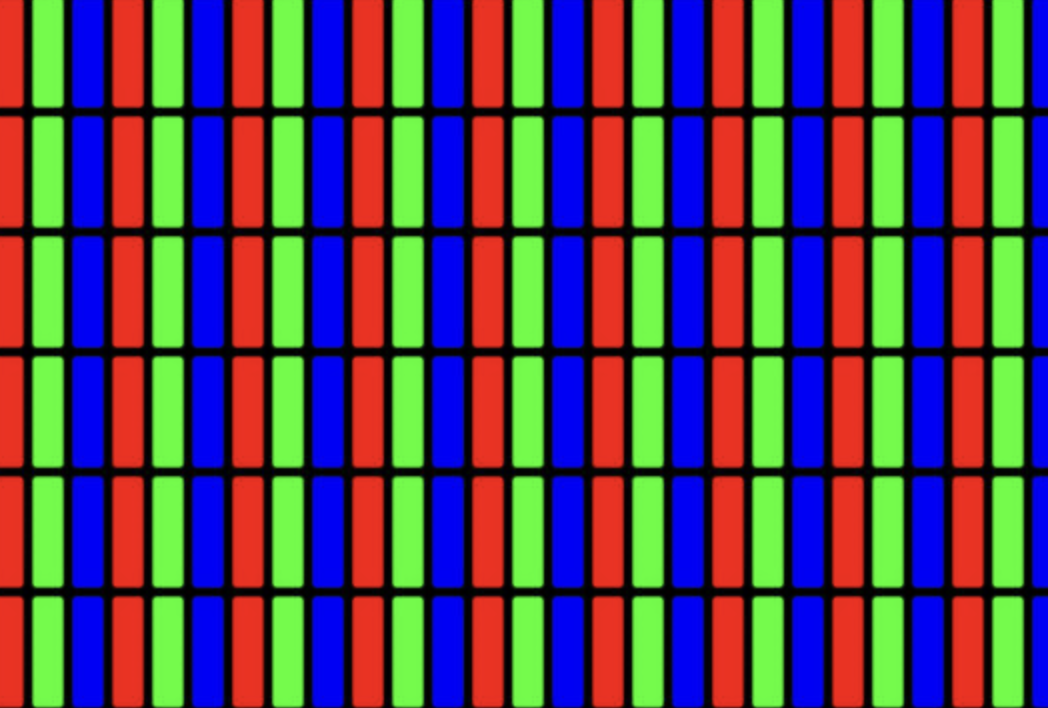
\includegraphics[width=0.3\linewidth]{Grundlagen_Info/01_TheoretischeInformatik/Figures/pixels}
	\caption{\gls{LED}-Leuchtmittel in einem Computer-Bildschirm}
	\label{fig:pixels}
\end{figure}


Durch die Mischung der jeweiligen Leucht-Intensitäten kann eine Vielzahl möglicher Farben dargestellt werden (siehe \cref{fig:rgb-farbmischung}).

\begin{figure}[H]
	\centering
	\begin{subfigure}{.49\textwidth}
		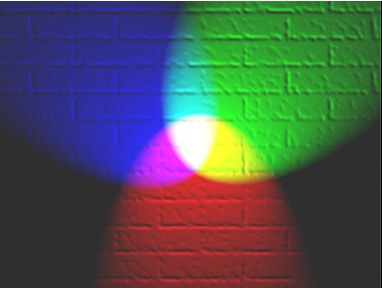
\includegraphics[width=\textwidth]{Grundlagen_Info/01_TheoretischeInformatik/Figures/rgb-farbmischung-1}
		\caption{Lichtkegel machen dasselbe wie ein Monitor}
		\label{fig:rgb-farbmischung-1}
	\end{subfigure}
	\begin{subfigure}{.49\textwidth}
		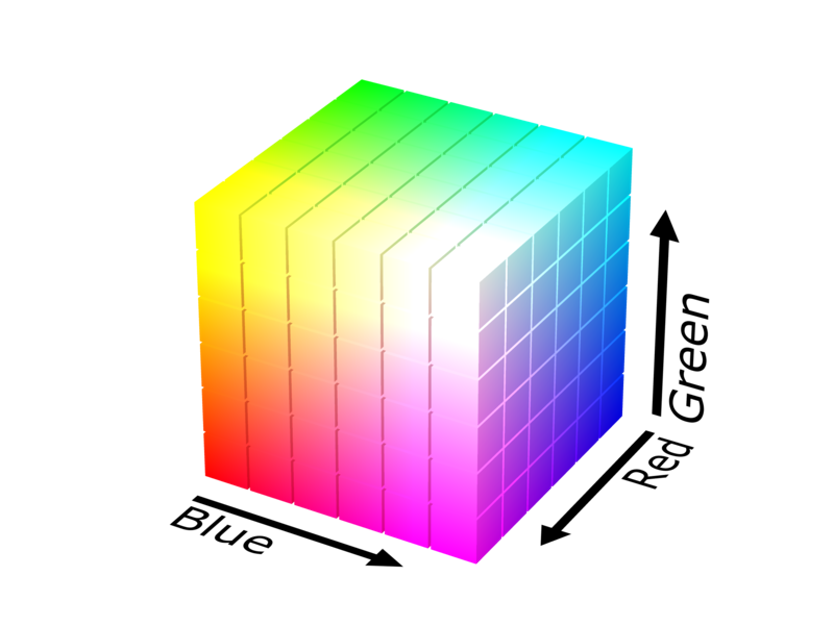
\includegraphics[width=\textwidth]{Grundlagen_Info/01_TheoretischeInformatik/Figures/rgb-farbmischung-2}
		\caption{Mögliche Farbmischungen}
		\label{fig:rgb-farbmischung-2}
	\end{subfigure}
	\caption{Prinzip der additiven Farbmischung in einem Computer-Monitor}
	\label{fig:rgb-farbmischung}
\end{figure}

Wie weiss nun ein Bildschirm, welche Pixel wie hell leuchten sollen? Auch hier gilt: Da Computer nur mit Nullen und Einsen arbeiten können, wird jedes Pixel mit einer Zahl angesteuert, die die Helligkeit in \% bezeichnet. Moderne Bildschirme können eine Vielzahl von Farben abbilden.

\begin{myexample}
Da jedes Farb-Pixel eines Bildschirms typischerweise in 256 Helligkeitsstufen leuchten kann, braucht es 8 Bits ($=$ ein Byte) pro Farbe, um die Helligkeitsstufe zu kodieren, da $2^8=256$. Da pro \enquote{gemischte} Farbe 3 Pixel leuchten, braucht es also $3\cdot 8$ Bits, d.h. 24 Bits, um eine Farbe zu kodieren. Daraus ergibt sich, dass ein Monitor auf jedem Pixel $2^{24} \approx 16.7$ Millionen Farben darstellen kann.
\end{myexample}

\begin{myexample}
Da die Darstellung einer Farbe im Binärsystem 24 Stellen braucht, braucht es etwas Zeit, um diese Darstellung zu lesen. Stattdessen wird häufig die hexadezimale Schreibweise verwendet:

\texttt{\red{11111111}\green{00000000}\blue{00000000} = \#\red{FF}\green{00}\blue{00} = \red{255}, \green{0}, \blue{0}} = reines Rot

\texttt{\red{10000000}\green{10000000}\blue{10000000} = \#\red{80}\green{80}\blue{80} = \red{128}, \green{128}, \blue{128}} = grau

Mit dem Hashtag (\texttt{\#}) vor der Farbe wird klargestellt, dass die Farbwerte als hexadezimale Zahlen dargestellt sind.
\end{myexample}

\begin{myexercise}
	Ordnen Sie die folgenden hexadezimalen Farbkodierungen den Farben zu:

	\begin{minipage}[c]{.2\textwidth}
		\begin{itemize}
			\item \texttt{\#FF0000}
			\item \texttt{\#00FF00}
			\item \texttt{\#0000FF}
			\item \texttt{\#000000}
			\item \texttt{\#FFFFFF}
		\end{itemize}
	\end{minipage}
	\begin{minipage}[c]{.2\textwidth}
		\begin{itemize}
			\item Schwarz
			\item Grün
			\item Blau
			\item Rot
			\item Weiss
		\end{itemize}
	\end{minipage}
\end{myexercise}

\begin{mychallenge}
	Erraten Sie weitere Farben unter \href{https://oinf.ch/interactive/farben-raten/}{diesem Link}.
\end{mychallenge}
Jedes Pixel besteht also aus 3 Farben, die jeweils mit einem Byte kodiert werden. Die Anzahl Bits pro Pixel bestimmt die \tib{Farbtiefe} eines Bilds (siehe \cref{fig:farbtiefe}).

\begin{figure}[H]
	\centering
	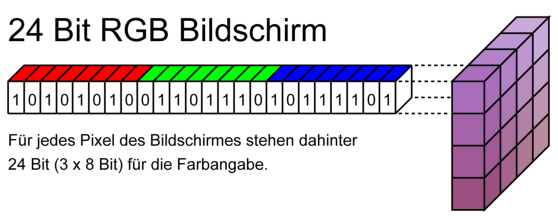
\includegraphics[width=0.7\linewidth]{Grundlagen_Info/01_TheoretischeInformatik/Figures/colordepth}
	\caption{Farbtiefe in einem Bild}
	\label{fig:farbtiefe}
\end{figure}

Je geringer die Farbtiefe, desto weniger fein können Farben oder Grautöne abgestuft werden (siehe \cref{fig:colordepth-examples}).

\begin{figure}[H]
	\centering
	\begin{subfigure}{.49\textwidth}
		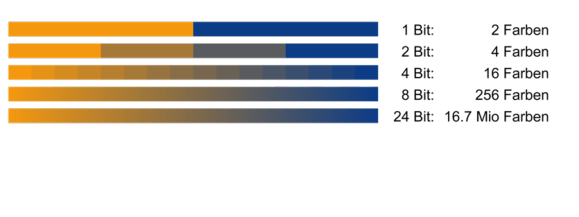
\includegraphics[width=\textwidth]{Grundlagen_Info/01_TheoretischeInformatik/Figures/colordepth-bar}
		\caption{Farbtiefe: Skala}
		\label{fig:colordepth-bar}
	\end{subfigure}
	\begin{subfigure}{.49\textwidth}
		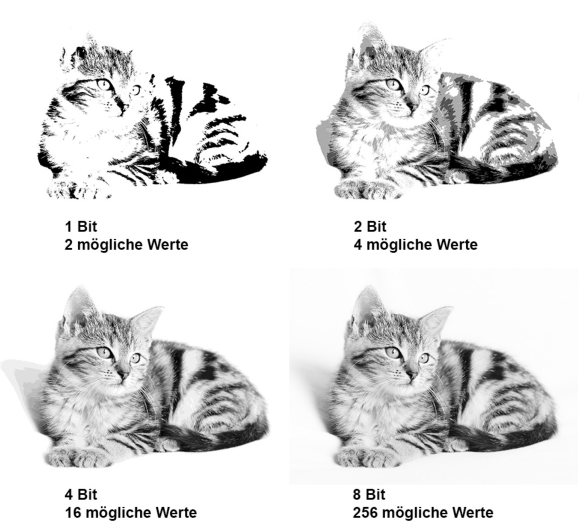
\includegraphics[width=\textwidth]{Grundlagen_Info/01_TheoretischeInformatik/Figures/colordepth-cat}
		\caption{Farbtiefen bei Graustufen-Bildern}
		\label{fig:colordepth-cat}
	\end{subfigure}
	\caption{Farbtiefe: Beispiele}
	\label{fig:colordepth-examples}
\end{figure}

Gewisse Bildformate sparen durch Indexierung und Kompression Speicherplatz. Falls beispielsweise ein grosser Teil des Bilds aus blauem Himmel besteht, muss die Farbe nicht für jedes einzelne Pixel abgespeichert werden. Mit dem Thema Kompression vertiefen wir uns in einem späteren Teil.

\begin{myexercise}
	Wie viel Speicherplatz braucht ein $500\cdot 500$ Pixel grosses Bild, wenn nur 64 Farben unterschieden werden sollen?
	\begin{myanswer}
		Das Bild hat 250'000 Pixel, und jedes Pixel braucht 6 Bit (da $2^6=64$). Das ergibt insgesamt $250'000\cdot 6 = 1'500'000$ Bits, oder umgerechnet $187'500$ Bytes ($=187.5$ KB).
	\end{myanswer}
\end{myexercise}

\section{Kodierung von weiteren Dateiformaten}
Wir wissen nun, dass Computer nur mit Nullen und Einsen \enquote{arbeiten}. Woher wissen wir aber, ob eine Folge aus Nullen und Einsen ein Bild, eine Zahl, ein Buchstabe oder etwas anderes repräsentiert? Hier kommen Dateiformate ins Spiel (siehe \cref{table:formats-codes}).

\begin{table}[H]
	\centering
	\begin{tabular}{l|p{11cm}}
		\textbf{In der Datei}           & \textbf{Bedeutung (z.B.)}                                                                                 \\\midrule
		\texttt{dateiname.\textbf{txt}} & die Zeichen: $<|\ldots$                                                                                   \\
		\texttt{dateiname.\textbf{doc}} & Teil des Befehls: \enquote{Einzug links um 1.75 cm}                                                       \\
		\texttt{dateiname.\textbf{xls}} & die Zahl 9662249 in einer Zelle                                                                           \\
		\texttt{dateiname.\textbf{gif}} & 3 Bildpunkte: blau, hellblau, weinrot (\texttt{.gif} kennt nur 256 Farben $\rightarrow$ 1 Byte pro Pixel) \\
		\texttt{dateiname.\textbf{bmp}} & 1 Bildpunkt: rötlich-braun (16.7 Mio. Farben $\rightarrow$ 3 Bytes pro Pixel)
	\end{tabular}
	\caption{Dateiformate und Kodierungen: Bedeutung einer Bitsequenz (z.B. \texttt{10010011   01101111   00101001
		})}
	\label{table:formats-codes}
\end{table}

\begin{myexercise}
	Um zu sehen, dass all Ihre Dateien tatsächlich nur aus Nullen oder Einsen bestehen, können Sie sich \href{https://moodle.ksimlee.ch/pluginfile.php/56580/mod_lesson/page_contents/2836/VideoXxdDemo.mov}{dieses Video} anschauen.
\end{myexercise}


\section{Speicherplatz und Speicherbedarf}
Wir haben bereits gelernt, dass ein Byte acht Bits entspricht. Heutzutage rechnen wir jedoch mit höheren Grössenordnungen (siehe \cref{table:daten-groessenordnungen}).

\begin{table}[H]
	\centering
	\begin{tabular}{@{}l|rr|l@{}}
		\toprule
		\textbf{Masseinheit} & \multicolumn{2}{l|}{\textbf{Dezimalsystem}} & Grössenordnung                                   \\ \midrule
		KB (Kilobyte)        & $10^3$ B(yte)                               & 1'000 B             & eine Text-Datei            \\
		MB (Megabyte)        & $10^6$ B                                    & 1'000'000 B         & eine Musik-Datei           \\
		GB (Gigabyte)        & $10^9$ B                                    & 1'000'000'000 B     & eine Video-Datei           \\
		TB (Terabyte)        & $10^{12}$ B                                 & 1'000'000'000'000 B & kleiner Firmen-Server      \\
		PB (Petabyte)        & $10^{15}$ B                                 & ...                 & Facebook-Server (Meta)     \\
		EB (Exabyte)         & $10^{18}$ B                                 & ...                 & alle CERN-Daten            \\
		ZB (Zettabyte)       & $10^{21}$ B                                 & ...                 & alle Daten ($\sim$ 100 ZB) \\
		YB (Yottabyte)       & $10^{24}$ B                                 & ...                 & $\approx 2030$?            \\ \bottomrule
	\end{tabular}
	\caption{Gängige Daten-Grössenordnungen in der Informatik (ein \textbf{B}yte = 8 \textbf{b}it)}
	\label{table:daten-groessenordnungen}
\end{table}

\begin{myexercise}
	Welches ist der übliche / gebräuchliche Name für ein \enquote{Megagramm}?
	\begin{myanswer}
		eine Tonne
	\end{myanswer}
\end{myexercise}

\begin{mychallenge}
	Weshalb haben Festplatten häufig eine leicht kleinere Speichergrösse als angegeben, insbesondere unter Windows? Lesen Sie dazu \href{https://support.apple.com/en-us/102119}{diesen Support-Artikel von Apple}.
\end{mychallenge}
